\section{Multi-Armed Bandit Problems}
\textbf{Setting:} A single state (aka situation) with multiple actions, one of which must be selected repeatedly. Each arm is slot machine with a stationary
probability distribution of rewards, say, $\mathcal{N}(\mu_i, \Sigma_i)$. The goal is to maximize the expected reward over some time horizon.

\begin{figure}[h]
    \centering
    
\includegraphics[width=0.9\textwidth]{img/bandit.png}
    \caption{A single state with multiple actions.}
    \label{fig:bandit}
\end{figure}


The expected reward of taking an action is given by:
\begin{equation}
    \begin{split}
        q_*(a) = \mathbb{E}[R_t | A_t = a] \\
        \label{eq:bandit}
    \end{split}
\end{equation}
This is the value of taking that action. We do not however know the value of each action, but we can estimate it by sampling the reward.
Thus, we approximate the value of an action as $Q_t(a) \approx q_*(a)$.

\subsection{Action-Value Methods}
Methods to estimate the value of an action and then use that estimate to select actions.

\subsubsection{Sample-Average Method:}
Each estimate is the average of all the sample of rewards collected up to that point.
\newline
Suppose $Q_t(a) = \frac{1}{N_t(a)} \sum_{i=1}^{N_t(a)} R_i$, where $N_t(a)$ is the number of times action $a$ has been selected up to time $t$.

\begin{equation}
    \begin{split}
        Q_t(a) = \frac{\sum_{i=1}^{t-1} R_i \cdot 1(A_i = a)}{\sum_{i=1}^{t-1} 1(A_i = a)} \\
        \label{eq:action-value}
    \end{split}
\end{equation}

\textbf{Action Selection:}
\begin{itemize}
    \item  Greedy: $ A_t = \text{argmax}_a Q_t(a) $
    \item  $\epsilon$-greedy: $ A_t = \begin{cases}
        \text{argmax}_a Q_t(a) & \text{with probability } 1 - \epsilon \\
        \text{random action} & \text{with probability } \epsilon
    \end{cases} $
\end{itemize}


With $\epsilon$-greedy, as $t \to \infty$, each action is sampled infinite times, and therefore the estimate $Q_t(a)$ converges to $q_*(a)$. 
The greedy selection, however, does not have strong convergence properties.

With `k' arms in  $\epsilon$-greedy method, the probability of selecting the greedy action is,
\begin{equation}
    \begin{split}
        P(\text{greedy action}) = (1 - \epsilon).P(\text{action is greedy}) + \epsilon.P(\text{action is random}) \\
        = (1 - \epsilon).1 + \epsilon.\frac{1}{k} \\
        = 1 - \epsilon + \frac{\epsilon}{k} \\
        \label{eq:epsilon-greedy}
    \end{split}
\end{equation}

The expected reward using $\epsilon$-greedy method is $(1 - \epsilon).q_*(a^*)$, because of the strong convergence
properties of the sample-average method. That is, in the long run, the expected reward will be equal to the expected
 value of selecting the greedy action.

 - If the variance of rewards increases across arms, it's always good to explore quickly. 
 $\epsilon$-greedy method is better than greedy method.

 - If the task is non-stationary, then the $\epsilon$-greedy method is good because we can explore previously explored
 actions whose rewards have potentially increased.
 \newline

\textbf{Incremental Implementation:}
\begin{equation}
    \begin{split}
        Q_{t+1}(a) = Q_t(a) + \frac{1}{N_t(a)} (R_t - Q_t(a)) \\
        \label{eq:incremental-implementation}
    \end{split}
\end{equation}

Simple bandit algorithm:
\begin{algorithm}
    \caption{Simple Bandit Algorithm}
    \begin{algorithmic}
        \State $Q(a) \leftarrow 0$
        \State $N(a) \leftarrow 0$
        \For{$t = 1$ to $T$}
            \State $A_t \leftarrow \begin{cases}
                \text{argmax}_a Q(a) & \text{with probability } 1 - \epsilon \\
                \text{random action} & \text{with probability } \epsilon
            \end{cases}$
            \State $R_t \leftarrow \text{reward}(A_t)$
            \State $Q(A_t) \leftarrow Q(A_t) + \frac{1}{N(A_t)} [R_t - Q(A_t)] $
            \State $N(A_t) \leftarrow N(A_t) + 1$
        \EndFor
    \end{algorithmic}
\end{algorithm}

\subsubsection{Non-Stationary Problems: Exponential Recency Weighting}

In the case of non-stationary problems, we would want to give more weight to recent rewards.
\begin{equation}
    \begin{split}
        Q_{t+1}(a) = Q_t(a) + \alpha [R_t - Q_t(a)] \\
        = (1 - \alpha)^t Q_1(a) + \sum_{i=1}^{t} \alpha (1 - \alpha)^{t-i} R_i \\
        \label{eq:non-stationary-implementation}
    \end{split}
\end{equation}

Note that all of the above methods are biased by the initial estimate $Q_1(a)$ (aka prior knowledge).
For sample average methods, the bias disappears once all actions are explored at least once. 
$Q_t(a) >> R_t$ allows us to explore the actions more quickly. Wild optimism is a good strategy.
For non-stationary problems, however, the bias is persistent but decreasing over time. So this drive for exploration is temporary.


\subsection{Gradient Bandit}
Instead of estimating the value of each action, we estimate the numerical preference for each action, $H_t(a)$.
With exact gradient ascent,

\begin{equation}
    \begin{split}
        H_{t+1}(a) = H_t(a) + \alpha \frac{\partial \mathbb{E}[R_t]}{\partial H_t(a)} \\
        \label{eq:gradient-bandit}
    \end{split}
\end{equation}
\begin{equation}
    \begin{split}
        \pi_t(A_t = a) = P(A_t = a) = \frac{e^{H_t(a)}}{\sum_{b=1}^{k} e^{H_t(b)}} \\
        \label{eq:gradient-bandit-policy}
    \end{split}
\end{equation}

Hence, $\mathbb{E}[R_t] = \sum_{x} \pi_t(x) q_*(x)$; Given that we do not know $q_*(x)$, we can show that
this is an instance of stochastic gradient ascent with robust convergence properties.

\begin{equation}
    \begin{split}
        H_{t+1}(a) = \begin{cases}
            H_t(a) + \alpha (R_t - R_{avg_t}) (1 - \pi_t(A_t)) & \text{if } a = A_t \\
            H_t(a) - \alpha (R_t - R_{avg_t}) \pi_t(a) &  \text{for all } a \neq A_t \\
        \end{cases} \\
        \label{eq:gradient-bandit-gradient}
    \end{split}
\end{equation}


\subsection{Contextual Bandits}


\begin{figure}[h]
    \centering
    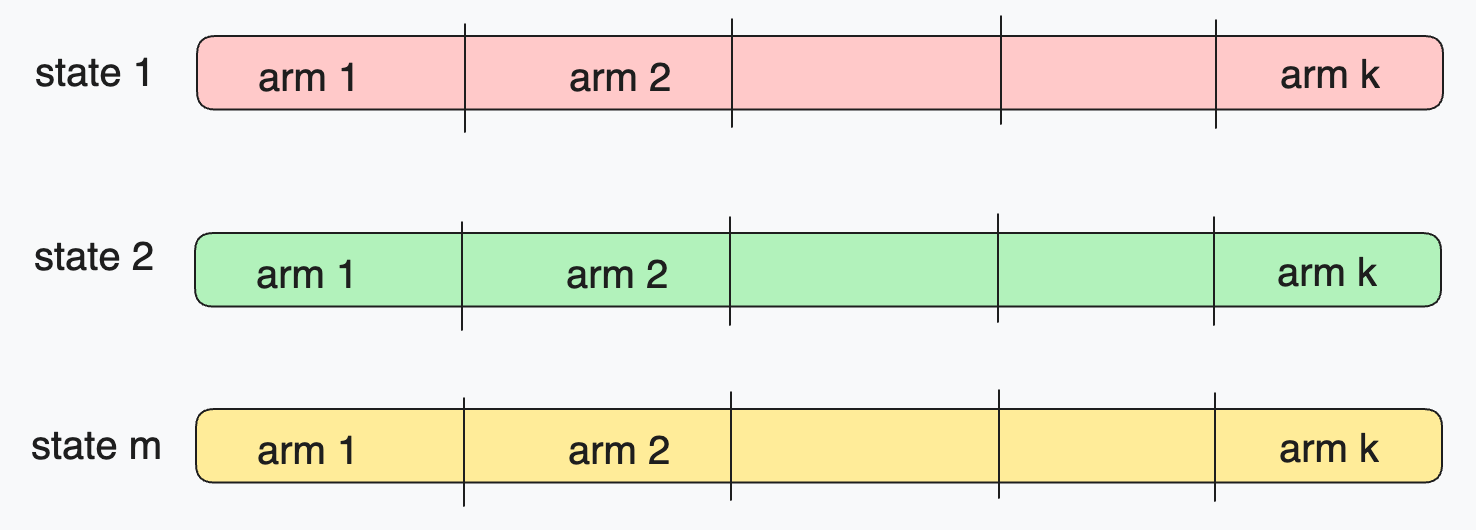
\includegraphics[width=0.9\textwidth]{img/contextual_bandit.png}
    \caption{Contextual Bandit with many states, each with multiple actions.}
    \label{fig:contextual-bandit}
\end{figure}

Associative search is a contextual bandit problem where we do trial-and-error learning to
\begin{itemize}
    \item  search for the best action, and,
    \item the association of these actions with the best situation (state) to be in.
\end{itemize}

Each $(s,a)$ pair results in a reward $R_{s,a}$. However, it does not change the state $s$.
If the state changes, we are in a full reinforcement learning problem.
